\begin{figure*}[htbp]
	\centering
	\caption{Visual comparison of Grad-CAM heatmaps under varying binarization thresholds $\tau \in \{0.5, 0.6, 0.7, 0.8\}$. The optimal threshold $\tau = 0.7$ isolates the core decision-relevant red/yellow regions without introducing peripheral noise ($\tau \le 0.6$) or truncating essential target features ($\tau = 0.8$).}
	\label{fig:threshold_comparison}
	\vskip 4pt
	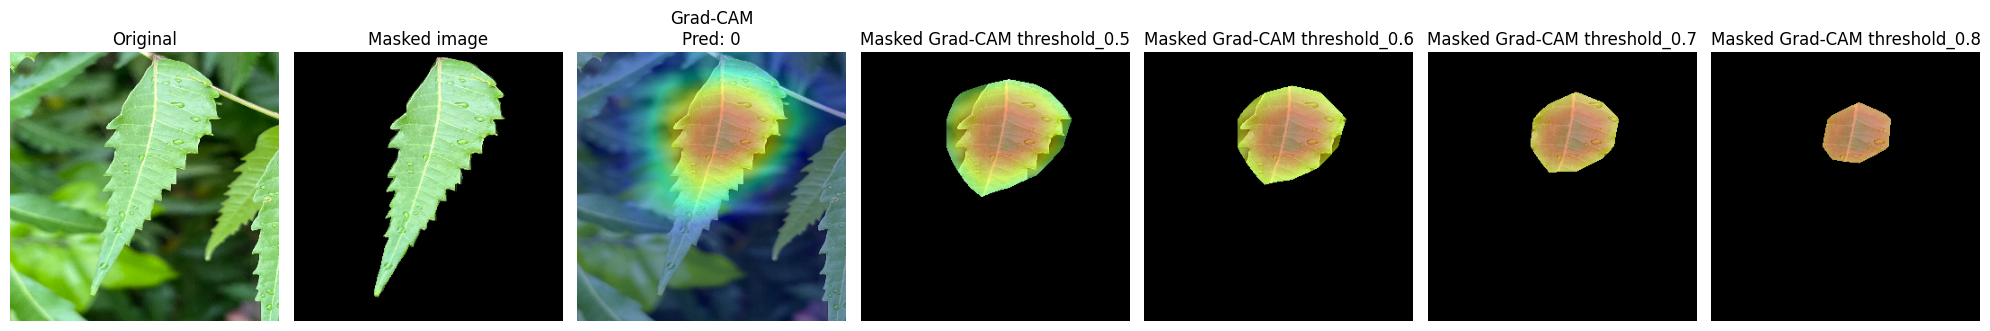
\includegraphics[width=0.98\textwidth]{figures/image.png}
	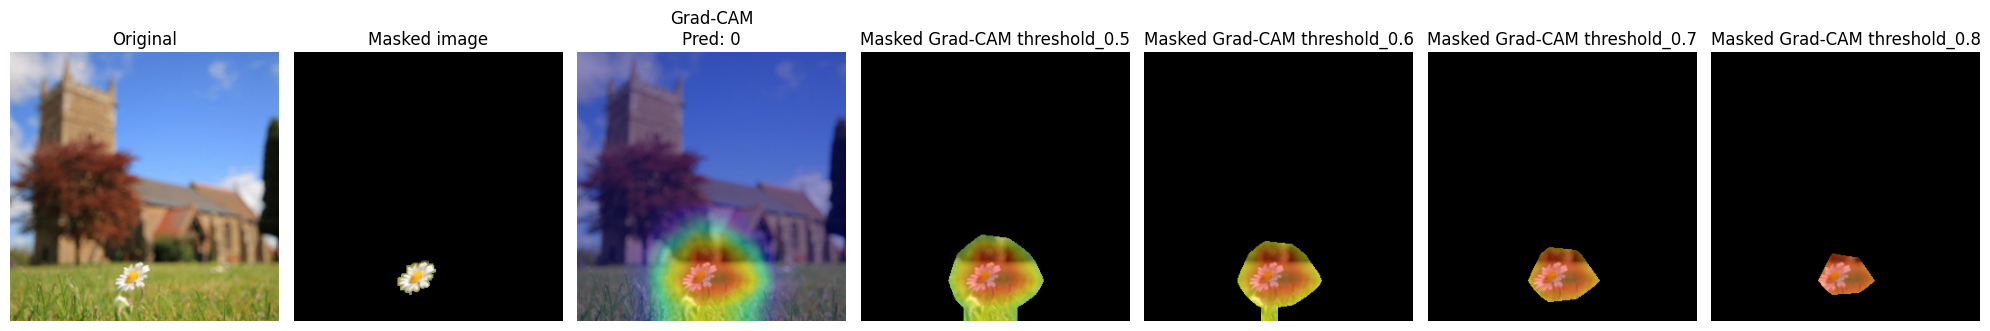
\includegraphics[width=0.98\textwidth]{figures/12.png}
	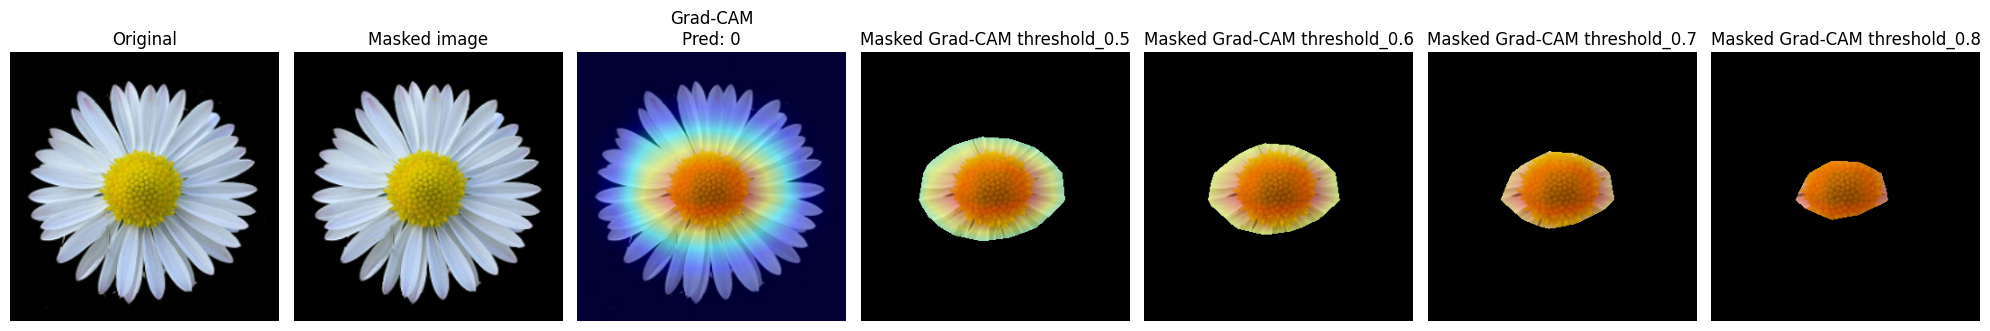
\includegraphics[width=0.98\textwidth]{figures/16.png}
	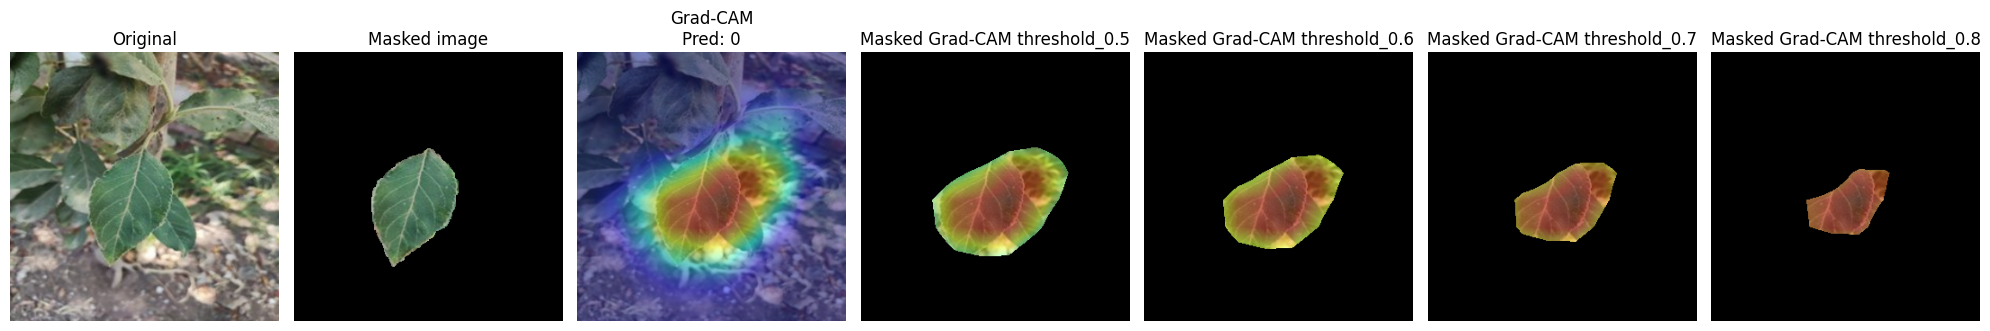
\includegraphics[width=0.98\textwidth]{figures/4.png}
\end{figure*}